%Cabeçalho
\documentclass[a4paper]{report}
%  \documentclass[opções]{estilo}
%	algumas opções são:
%		10pt, 11pt ou 12pt para o tamanho base das letras do texto.
%		a4paper ou letter para o tamanho do papel.
%		landscape ou portrait para orientação do papel para impressão
%	o estilo pode ser: article, report, book ou letter

%Pacotes
\usepackage [utf8] {inputenc} %codificação de entrada de caracteres
\usepackage [english] {babel} %dicionário pt-br
\usepackage[top=2cm, bottom=2cm, left=3cm, right=2cm]{geometry}
\usepackage[T1]{fontenc}
\usepackage{amsmath}
\usepackage{amsfonts}
\usepackage{amssymb}
\usepackage{graphicx}
\usepackage{ifthen}

%\pagestyle{empty} %Retira o número da página

\DeclareMathOperator{\sen}{sen} 
\DeclareMathOperator{\tg}{tg}

\newcommand {\resp}[2]{
	\vspace{0.4cm}\\
	Resposta: #1\\
	\if&#2&
	
	\else
		\\Resultado: #2
	\fi	
	\vspace{0.4cm}
}

%Documento
\begin{document}

\begin{center}
UNIVERSIDADE FEDERAL DO ESPÍRITO SANTO\\DEPARTAMENTO DE MATEMÁTICA\\
\vspace{0.6cm}
Solução dos exercícios do Capítulo 7
\vspace{0.2cm}

\end{center}
Seção 7.8:
\begin{enumerate}
		\item Questão 8:\\Seja $x$ a idade de Maria e $y$ a de seu filho quando o produto de suas idades era igual à $203$, ou seja $xy=203$. Se Maria teve seu filho aos 22 anos de idade, a idade de Maria, quando o produto das idades era 203, é dada por $x = 22 + y$. Logo, $x.y = (22 + y)y = 203$. Assim, temos que $y^2 + 23y - 203 = 0$, o que nos dá $y = -29$ e $y = 7$. Como a idade é sempre posivitiva a resposta é $y = 7$.
		
		\item Questão 9:\\Como um lado da cerca será a parede de armazém existente, a cerca de $50 m$ deve cercar apenas $3$ lados do retângulo formado. Sendo $x$ e $y$ os lados do retângulo formado pela cerca e a parede do armazém, temos que $2x+y=50$ e sua área cercada é dada por $S = x.y$. Daí $S = x.(50 - 2x) = 50x - 2x^2$. Como S em função de x é uma parábola com concavidade para baixo, podemos afirmar que existe um valor máximo para S e é dado por $x=\cfrac{-50}{2\times(-2)} = 12,5$. Logo, $y = 50 - 2\times12,5 = 25$. Portanto o retângulo cercado tem dimensões $12,5\times 25$ m.

		\item Questão 10:\\Utilizando o Teorema de Pitágoras no triangulo $AA'D'$, temos que o lado do quadrado circunscrito é dado por $y=\sqrt{x^2+ (10-x)^2}$ e sua área por $S = y^2 = x^2+ (10-x)^2 = 2x^2-20x+100$. Sendo S uma função de x uma parábola com concavidade para cima, podemos afirmar que o ponto que dá área mínima é $x=\cfrac{-(-20)}{2\times2}=5$ m.
		
		{
			\begin{figure}[!th]
				\centering
			 	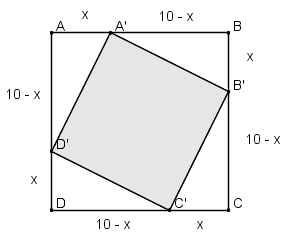
\includegraphics[height=0.3\linewidth]{q10.png}
			\end{figure}
		}	

		\item Questão 11:\\A pista de atletismo terá a forma mostrada na figura abaixo. Portanto, seu perímetro será dado por $2C + 2\pi R = 400$  e a área do campo de futebol será $S = 2CR$. Substituindo o valor de C, obtido pela equação do perímetro, em $S$, temos que $S=(400-2\pi R)R=400R-2\pi  R^2$. Sendo $S$ em função de $R$ côncava para baixo, o valor de R para qual $S$ será máximo é dado por $R=\cfrac{-400}{2(-2\pi)}=\cfrac{100}{\pi}$ m. Portanto, $C = \cfrac{400-\cfrac{2\pi 100}{\pi}}{2}=100$ m e o campo tem dimensões $100\times\cfrac{200}{\pi}$ m.

		{
			\begin{figure}[!t]
				\centering
			 	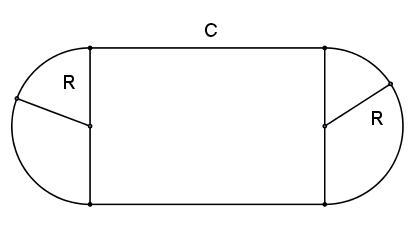
\includegraphics[height=0.2\linewidth]{q11.png}
			\end{figure}
		}	

		\item Questão 12:\\ O perímetro da cerca (apenas uma volta) é dado por $p=2r+\theta r = \cfrac{360}{3}=120$, logo $\theta = \cfrac{120-2r}{r}$. A área cercada $S$ é dada em função de $r$ por $S=\cfrac{\theta r^2}{2}=\cfrac{(120-2r)r^2}{2r}=60r-r^2$. Sendo $S$ um parábola côncava para baixo, seu ponto de máximo ocorre quando $r=\cfrac{-60}{-2}=30$ m. Portanto a área máxima será de $S=900$ m$^2$.

		{
			\begin{figure}[!th]
				\centering
			 	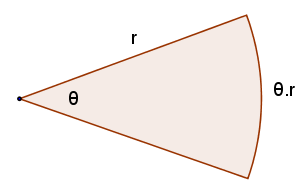
\includegraphics[height=0.2\linewidth]{q12.png}
			\end{figure}
		}	

		\item Questão 13:\\ A soma da área das duas figuras formadas pelos dois pedaços de arame é dada por $S = \pi r^2 + L^2$, onde $r=\cfrac{x}{2\pi}$ e $L = \cfrac{(1-x)}{4}$. Portanto $S=\cfrac{(4+\pi)x^2-2\pi x+\pi}{16\pi}$. Sendo S côncava para cima, temos de imediato que $x=\cfrac{-(-2\pi)}{2(4+\pi)}$  nos dá o ponto onde S é mínimo. Além disso, poderíamos pensar que $S$ não possui valor máximo, no entanto, a variável x está limitada entre 0 e 1 m, logo o ponto de máximo será dado quando $x =0$ ou $x=1$. Para $x=0$ temos $S(0) = \cfrac{1}{16}$ e para $x=1$ temos $S(1)=\cfrac{1}{4\pi}$. Como $S(1) > S(0)$, temos que $x=1$ é o ponto procurado. Portanto, os pedaços que dão área máxima e mínima são $(1,0)$ e $(\cfrac{\pi}{4+\pi}, \cfrac{4}{4+\pi})$, respectivamente.

		{
			\begin{figure}[!th]
				\centering
			 	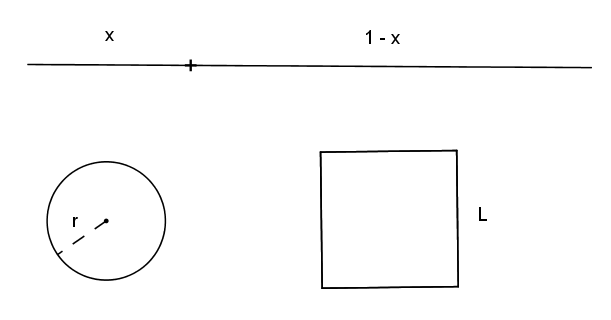
\includegraphics[height=0.3\linewidth]{q13.png}
			\end{figure}
		}	

		\item Questão 14:\\ A janela normanda está representada na figura abaixo. Para que a maior quantidade de luz passe por ela, suas dimensões devem ser tais que a área da janela seja máxima. A área $S$ da janela é dada por $hL + \cfrac{\pi L^2}{8}$ e seu perímetro $p$ por $2h+L+\cfrac{\pi L}{2}$. Colocando $h$ em função de $p$ e $L$ e substituindo em $S$, teremos $S=\cfrac{4pL-(4+\pi)L^2}{8}$. Sendo $S$ côncava para baixo, temos o ponto de máximo dado por $L=\cfrac{-4p}{-2(4+\pi)}=\cfrac{2p}{4+\pi}$, portanto $h=\cfrac{p}{4+\pi}$ e a janela terá dimensões $\cfrac{2p}{4+\pi} \times \cfrac{p}{4+\pi}$

		{
			\begin{figure}[!th]
				\centering
			 	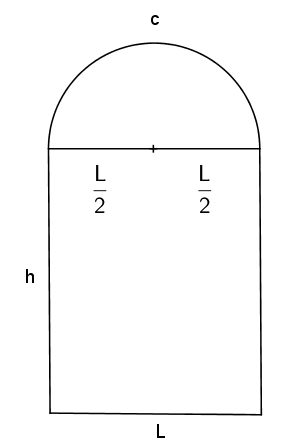
\includegraphics[height=0.3\linewidth]{q14.png}
			\end{figure}
		}

		\item Questão 15:\\ Seja $x$ a quantidade de alunos que irão viajar e $R(x)$ a função que dá a receita que o proprietário do ônibus terá. Se $x$ alunos irão viajar, restarão $50-x$ acentos vazios. Conforme combinado, a receita será dada por $80$ reais por lugar ocupado mais $5$ reais por acento vazio por aluno que irá viajar, portanto $R(x) = 80x+5x(50-x)= 330x-5x^2$. Sendo $S(x)$ côncava para baixo, o número de acentos ocupados que dará receita máxima será $x=\cfrac{-330}{-2\times5}=33$.

\end{enumerate}

\end{document}
